
\documentclass{beamer}
\usecolortheme{dove}
\setbeamertemplate{navigation symbols}{}
\usepackage{amsmath,amssymb,amsfonts,amsthm, multicol, subfigure, color}
\usepackage{bm}
\usepackage{graphicx}
\usepackage{tabularx}
\usepackage{booktabs}
\usepackage{hyperref}
\usepackage{pdfpages}
\usepackage{xcolor}
\definecolor{seagreen}{RGB}{46, 139, 87}
\definecolor{mustard}{RGB}{234, 170, 0}
\def\independenT#1#2{\mathrel{\rlap{$#1#2$}\mkern2mu{#1#2}}}
\newcommand\indep{\protect\mathpalette{\protect\independenT}{\perp}}
\def\log{\text{log}}
\newcommand\logit{\text{logit}}
\newcommand\iid{\stackrel{\text{iid}}{\sim}}
\newcommand\E{\text{E}}
\newcommand\V{\text{V}}
\renewcommand\P{\text{P}}
\newcommand{\Cov}{\text{Cov}}
\newcommand{\Cor}{\text{Cor}}
\newcommand\doop{\texttt{do}}
\usepackage{stackrel}
\usepackage{tikz}
\usetikzlibrary{arrows,shapes.arrows,positioning,shapes,patterns,calc}
\newcommand\slideref[1]{\vskip .1cm \tiny \textcolor{gray}{{#1}}}
\newcommand\red[1]{\color{red}#1}
\newcommand\blue[1]{\color{blue}#1}
\newcommand\gray[1]{\color{gray}#1}
\newcommand\seagreen[1]{\color{seagreen}#1}
\newcommand\purple[1]{\color{purple}#1}
\newcommand\orange[1]{\color{orange}#1}
\newcommand\black[1]{\color{black}#1}
\newcommand\white[1]{\color{white}#1}
\newcommand\teal[1]{\color{teal}#1}
\newcommand\magenta[1]{\color{magenta}#1}
\newcommand\Fuchsia[1]{\color{Fuchsia}#1}
\newcommand\BlueGreen[1]{\color{BlueGreen}#1}
\newcommand\bblue[1]{\textcolor{blue}{\textbf{#1}}}
\newcommand\bred[1]{\textcolor{red}{\textbf{#1}}}
\newcommand\bgray[1]{\textcolor{gray}{\textbf{#1}}}
\newcommand\bgreen[1]{\textcolor{seagreen}{\textbf{#1}}}
\newcommand\bref[2]{\href{#1}{\color{blue}{#2}}}
\colorlet{lightgray}{gray!40}
\pgfdeclarelayer{bg}    % declare background layer for tikz
\pgfsetlayers{bg,main} % order layers for tikz
\newcommand\mycite[1]{\begin{scriptsize}\textcolor{darkgray}{(#1)}\end{scriptsize}}
\newcommand{\tcframe}{\frame{
%\small{
\only<1|handout:0>{\tableofcontents}
\only<2|handout:1>{\tableofcontents[currentsubsection]}}
%}
}

\newcommand{\goalsframe}{\begin{frame}{Learning goals for today}
By the end of class, you will be able to
\begin{itemize}
    \item trace political origins of racial wealth inequality
    \item link these to data science questions with a
    \begin{itemize}
    \item unit of analysis
    \item set of predictors
    \item outcome variable
    \end{itemize}
\end{itemize} \vskip .2in
\end{frame}}

\usepackage[round]{natbib}
\bibliographystyle{humannat-mod}
\setbeamertemplate{enumerate items}[default]
\usepackage{mathtools}

\title{Studying Social Inequality with Data Science}
\author{Ian Lundberg}
\date{\today}

\begin{document}

\begin{frame}
\begin{tikzpicture}[x = \textwidth, y = \textheight]
\node at (0,0) {};
\node at (1,1) {};
\node[anchor = north west, align = left, font = \huge] at (0,.9) {Studying\\Social Inequality\\with Data Science};
\node[anchor = north east, align = right] (number) at (1,.9) {INFO 3370 / 5371\\Spring 2023};
\node[anchor = north, font = \Large, align = right] at (.5,.5) {\bblue{Political Origins of Wealth Inequality}};
\end{tikzpicture}
\end{frame}

\goalsframe

\begin{frame}
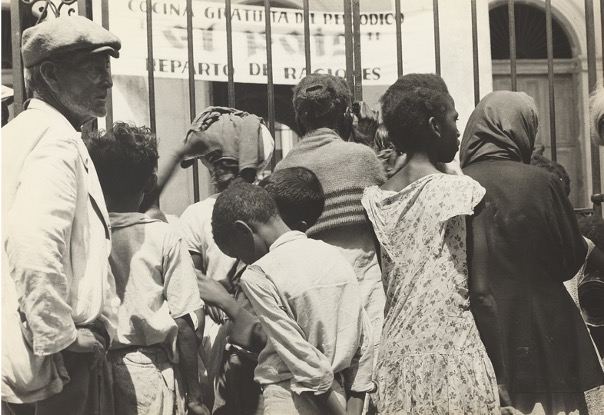
\includegraphics[height = .8\textheight]{figures/breadline}\\
\begin{footnotesize}
Walker Evans, 1933. The Breadline.\\
Source: \href{https://www.nga.gov/learn/teachers/lessons-activities/uncovering-america/great-depression.html}{National Gallery of Art}
\end{footnotesize}
\end{frame}

\begin{frame}
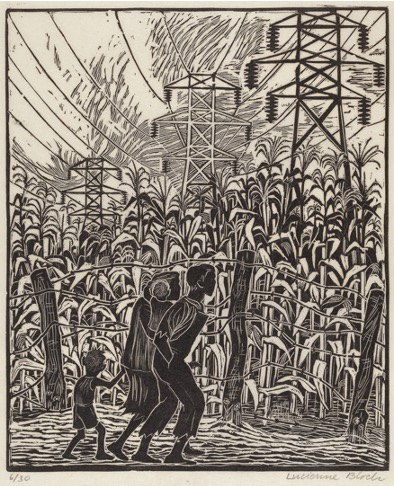
\includegraphics[height = .8\textheight]{figures/land_of_plenty}\\
\begin{footnotesize}
Lucienne Bloch, 1936. Land of Plenty.\\
Source: \href{https://www.nga.gov/learn/teachers/lessons-activities/uncovering-america/great-depression.html}{National Gallery of Art}
\end{footnotesize}
\end{frame}

\begin{frame}
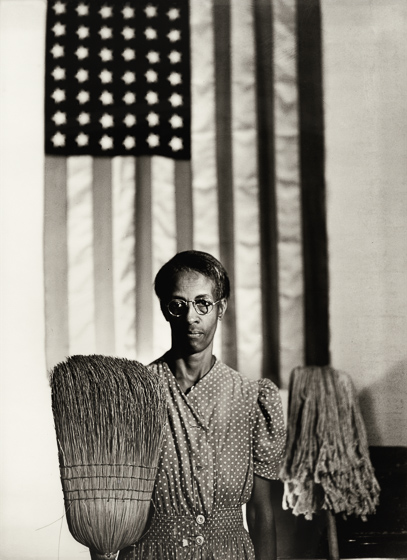
\includegraphics[height = .85\textheight]{figures/Parks-Charwoman-WSS}\\
\begin{footnotesize}
Gordon Parks, 1942. Washington, D.C. Government Charwoman (American Gothic).\\
Source: \href{https://www.nga.gov/learn/teachers/lessons-activities/uncovering-america/great-depression.html}{National Gallery of Art}
\end{footnotesize}
\end{frame}

\begin{frame}
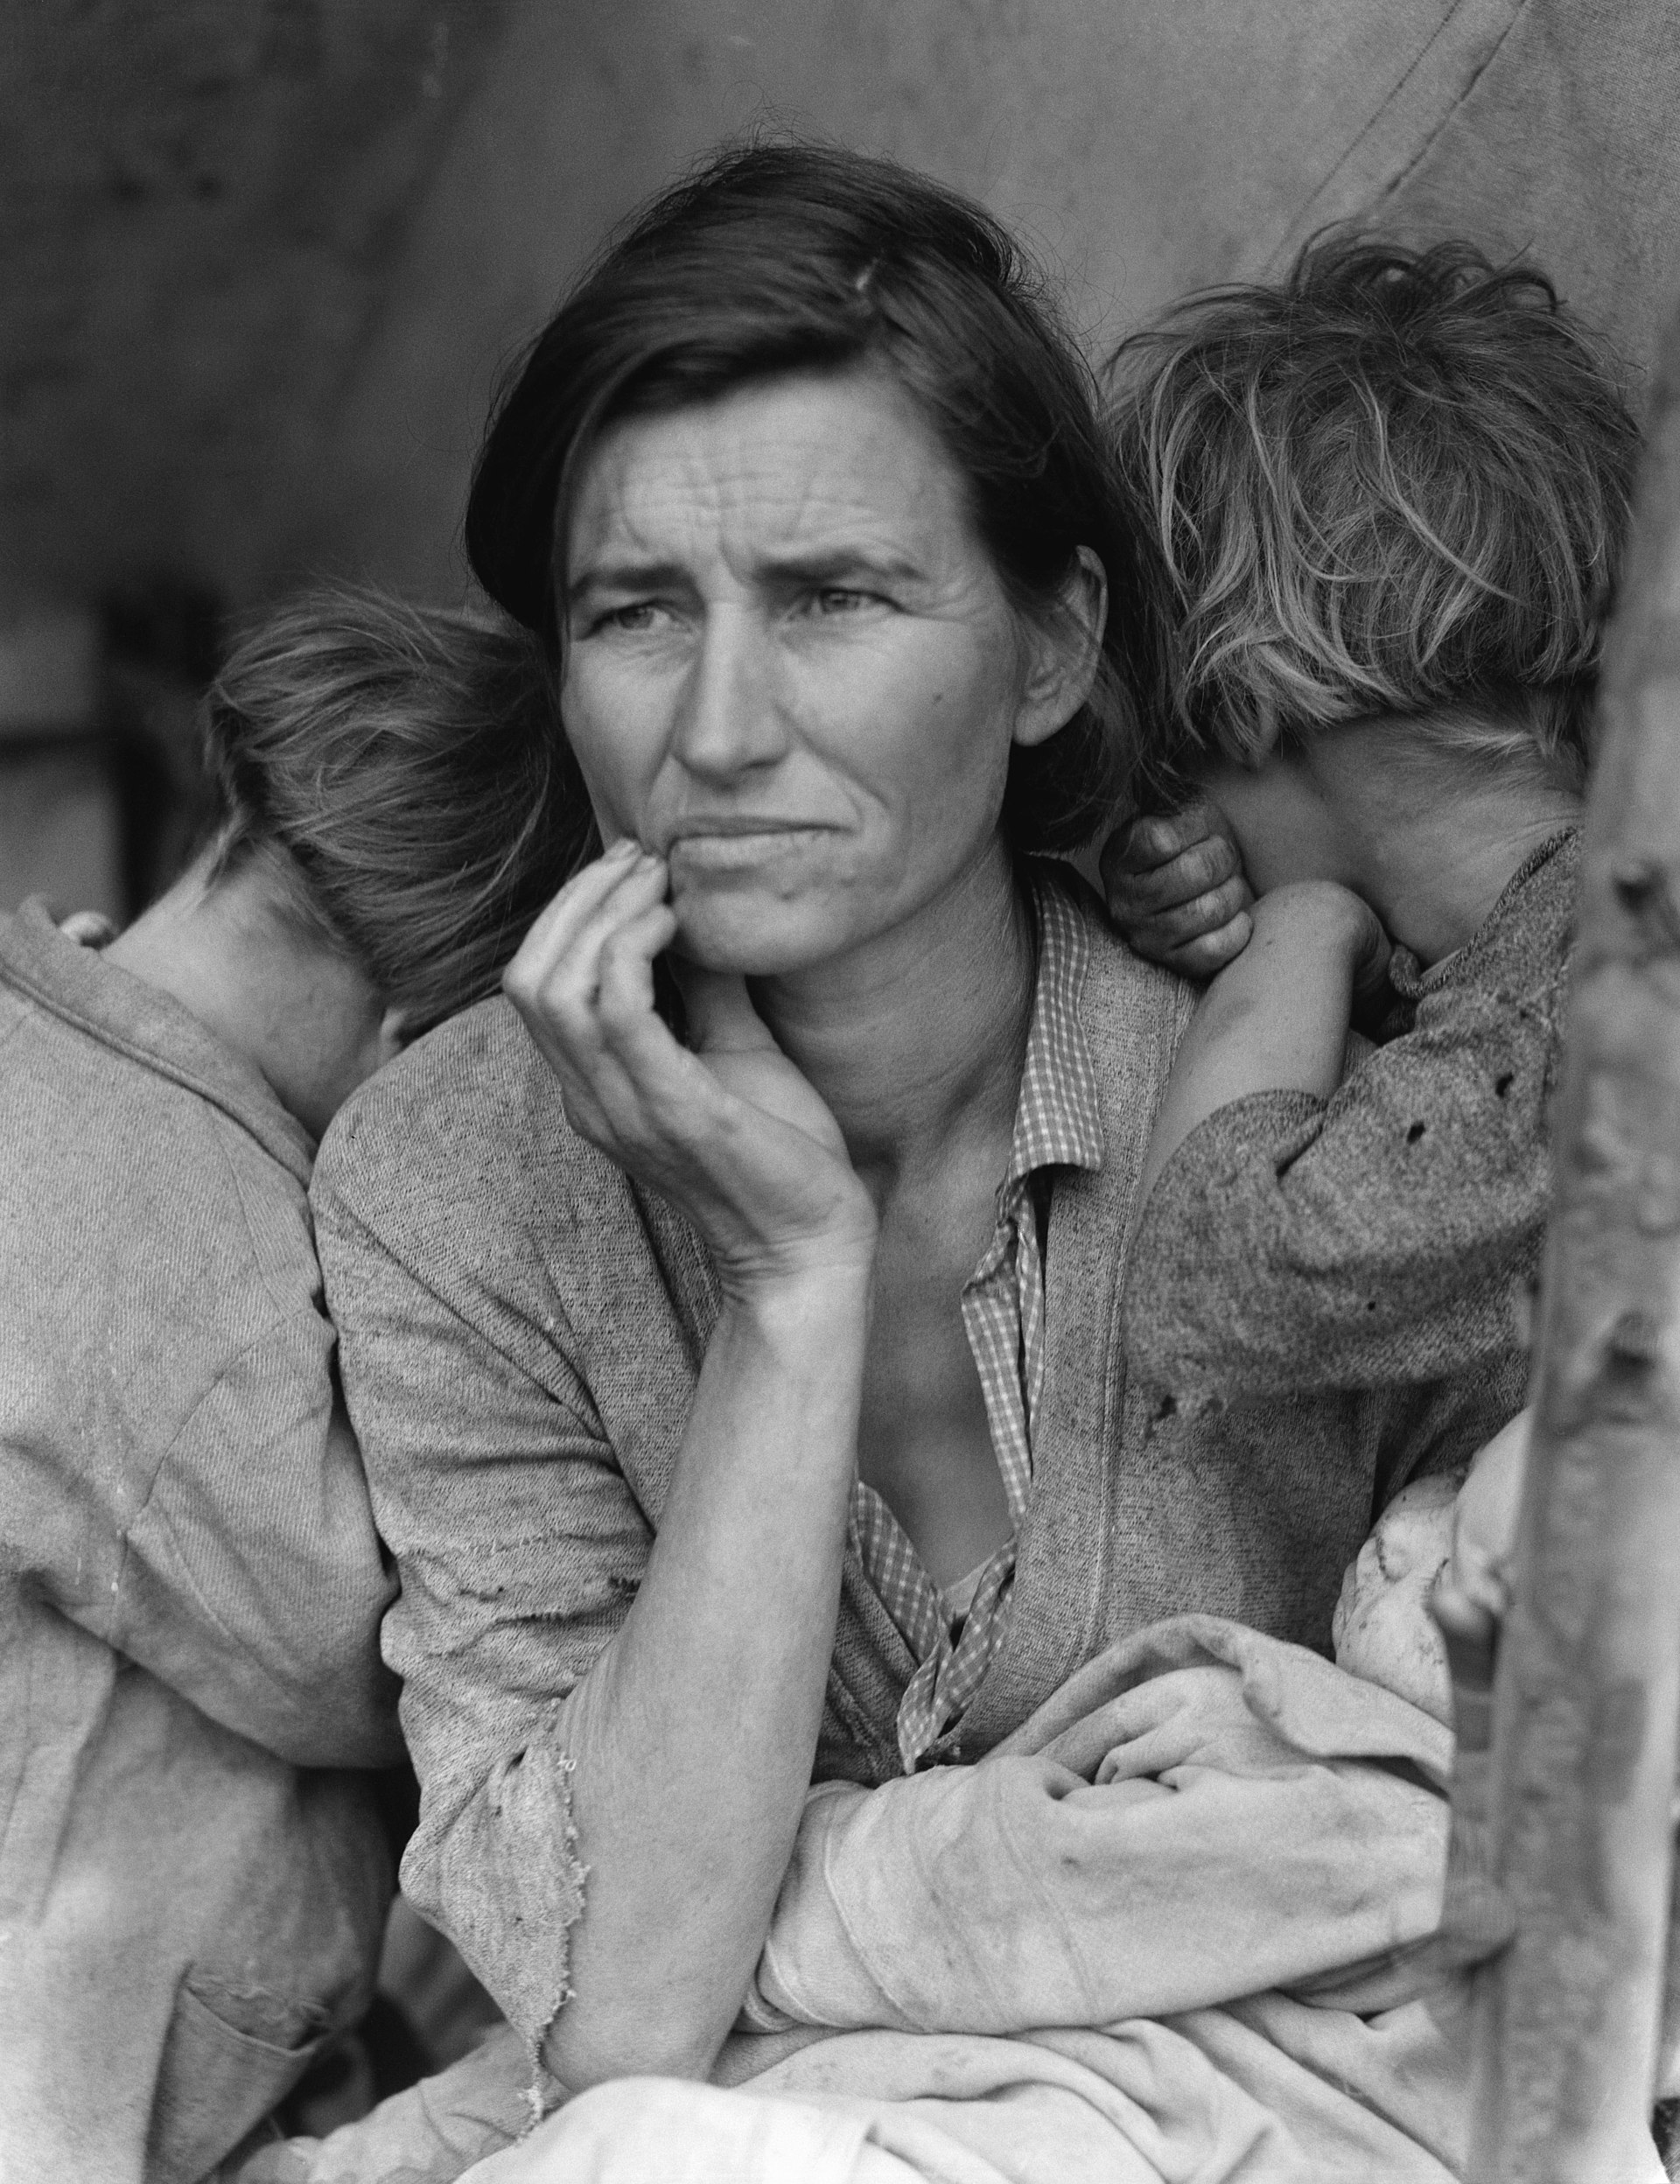
\includegraphics[height = .85\textheight]{figures/Lange-MigrantMother}\\
\begin{footnotesize}
Dorothea Lange, 1936. Migrant Mother.\\
Source: \href{https://en.wikipedia.org/wiki/Migrant_Mother}{Wikimedia}, original in MOMA NY
\end{footnotesize}
\end{frame}

\begin{frame}
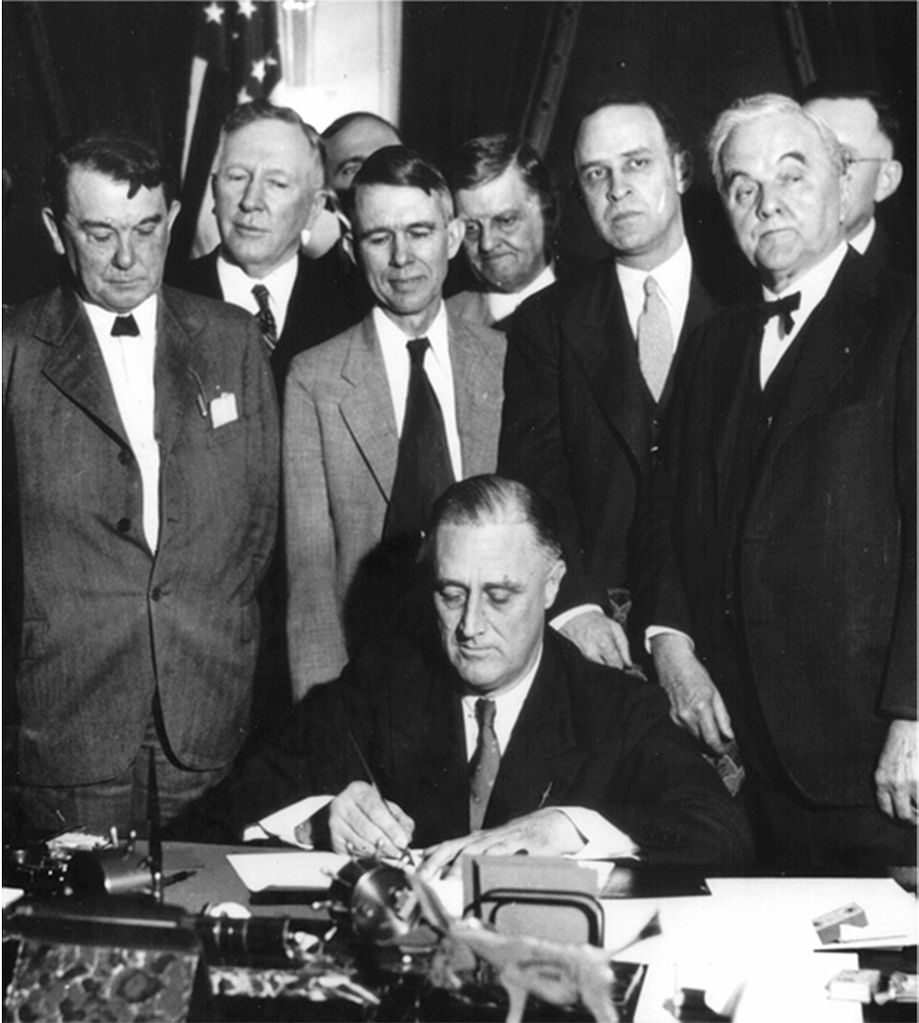
\includegraphics[width = .7\textwidth]{figures/fdr_tva}\\
Source: \href{https://commons.wikimedia.org/wiki/File:Roosevelt_signing_TVA_Act_(1933).jpg}{Wikimedia}
\end{frame}

\begin{frame}
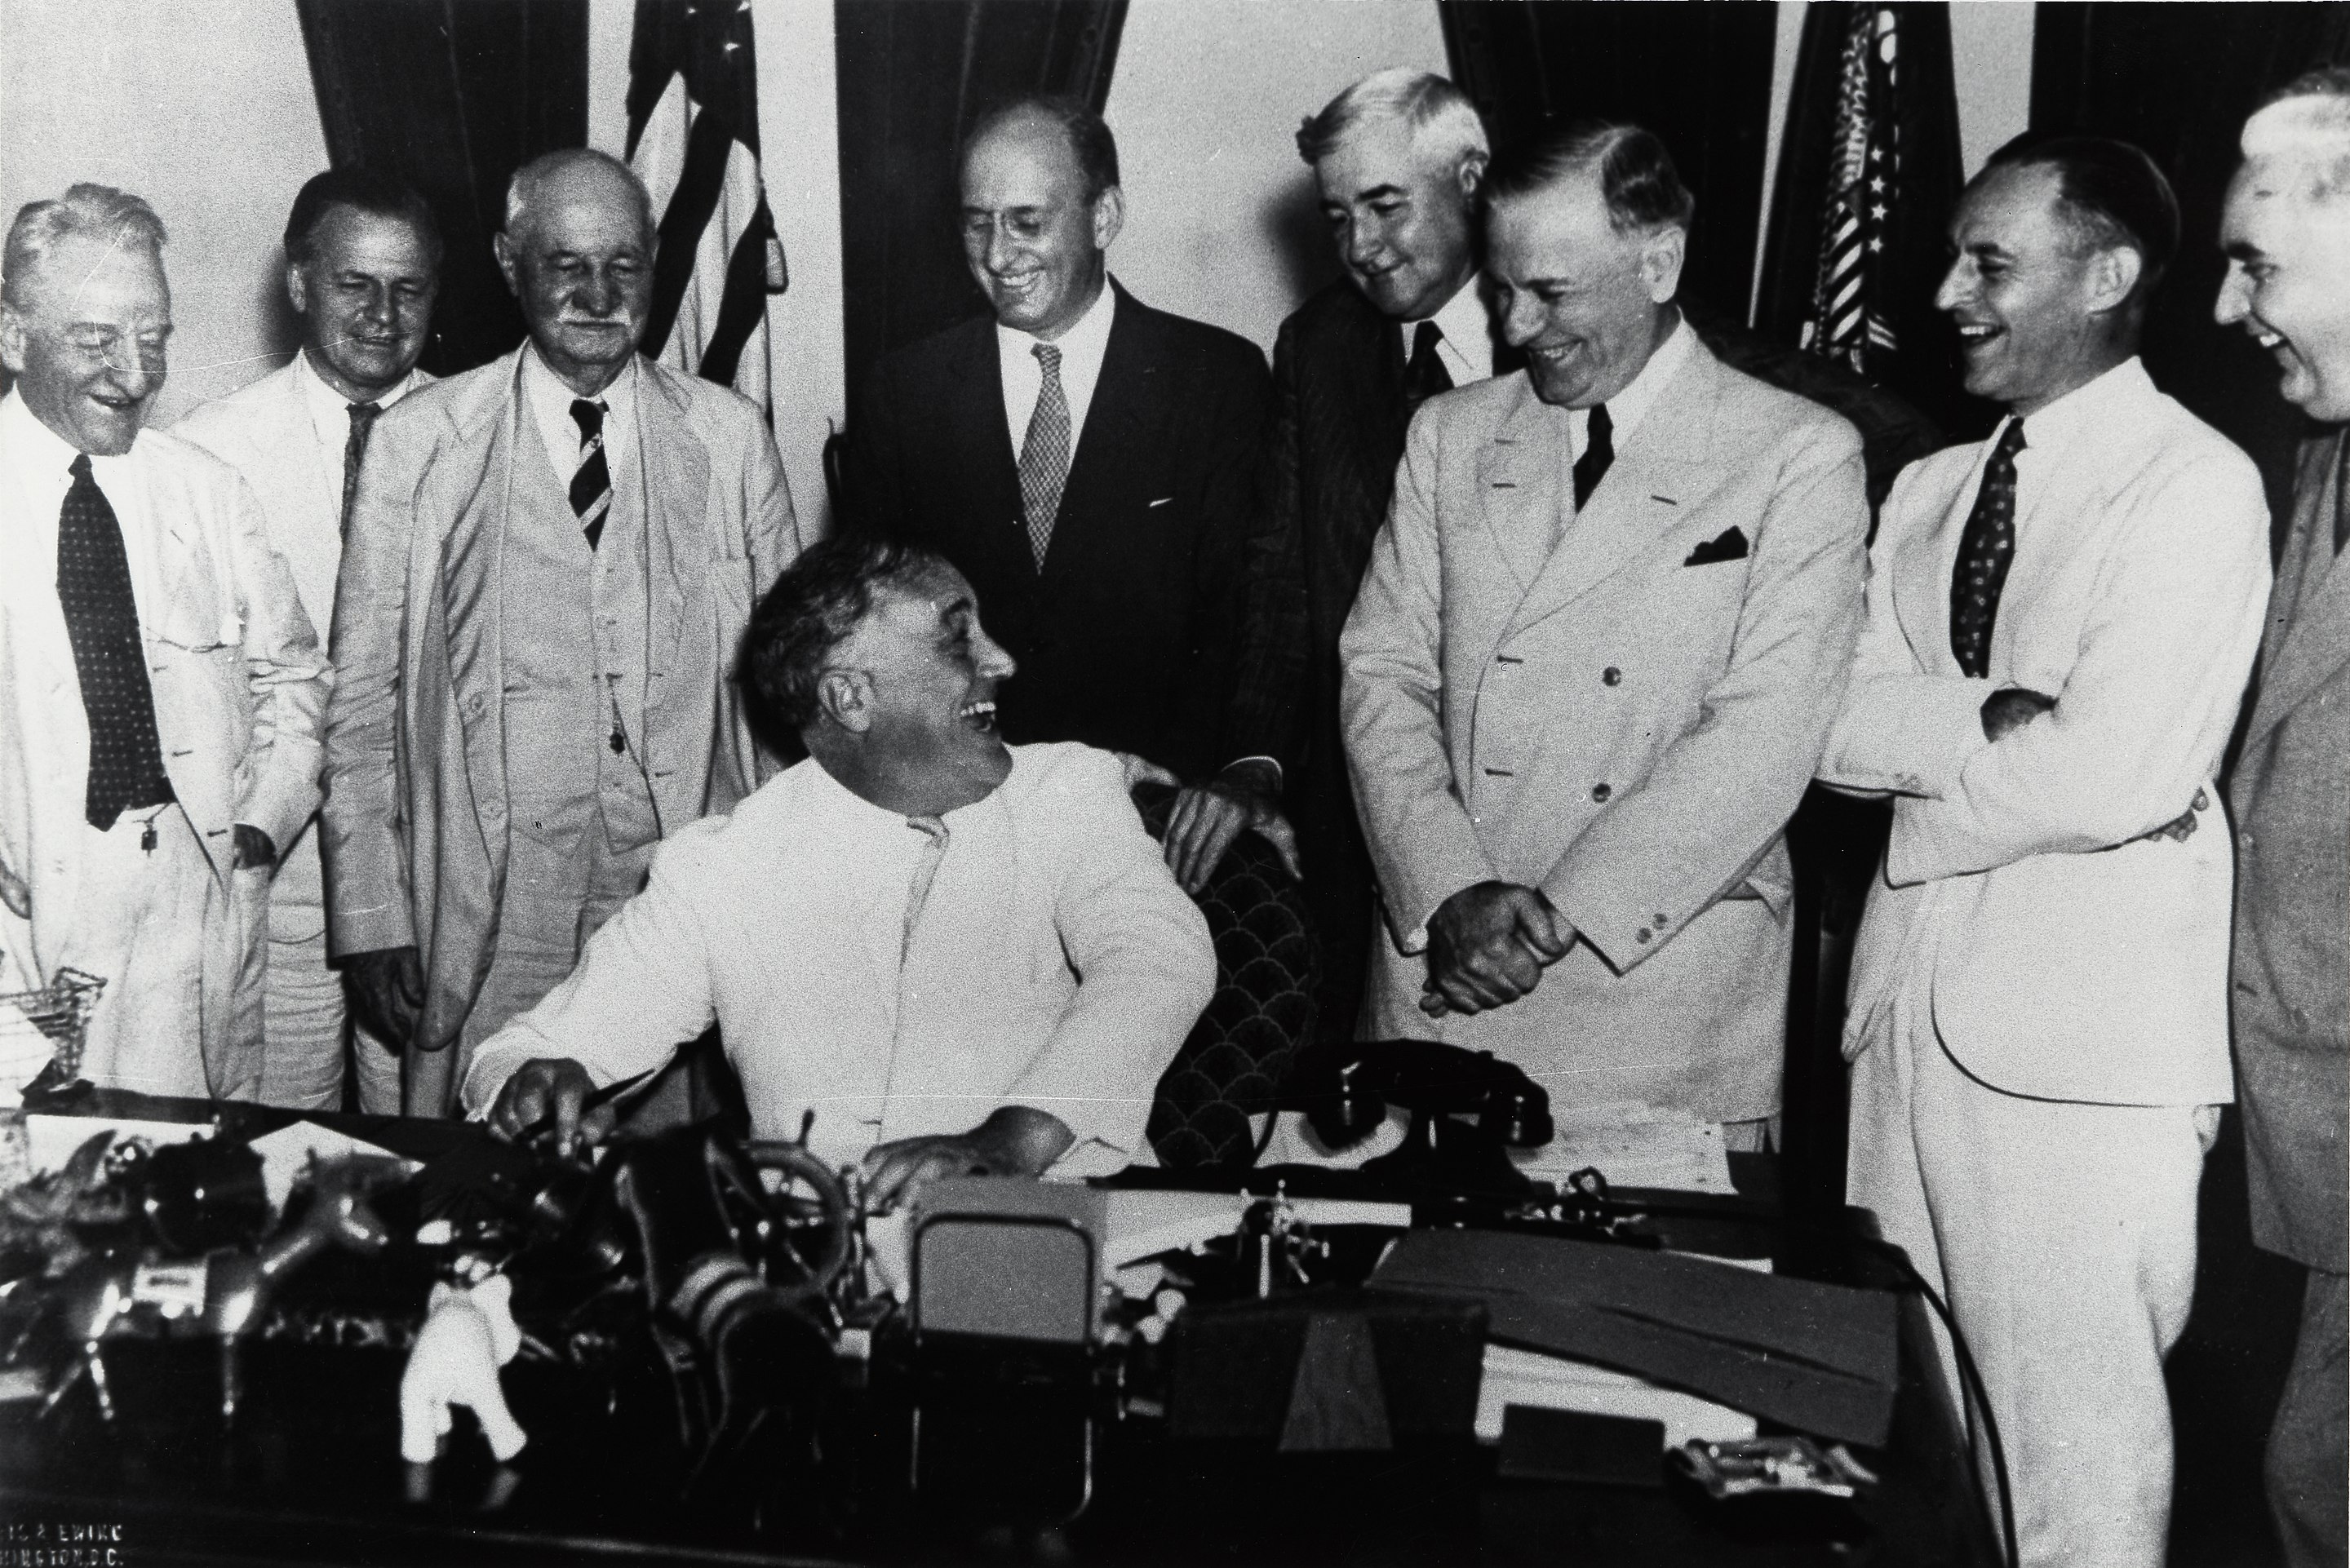
\includegraphics[width = .7\textwidth]{figures/fdr_banking}\\
Source: \href{https://commons.wikimedia.org/wiki/File:Franklin_Delano_Roosevelt_signs_Banking_Act_of_1935.jpg}{Wikimedia}
\end{frame}

\begin{frame}
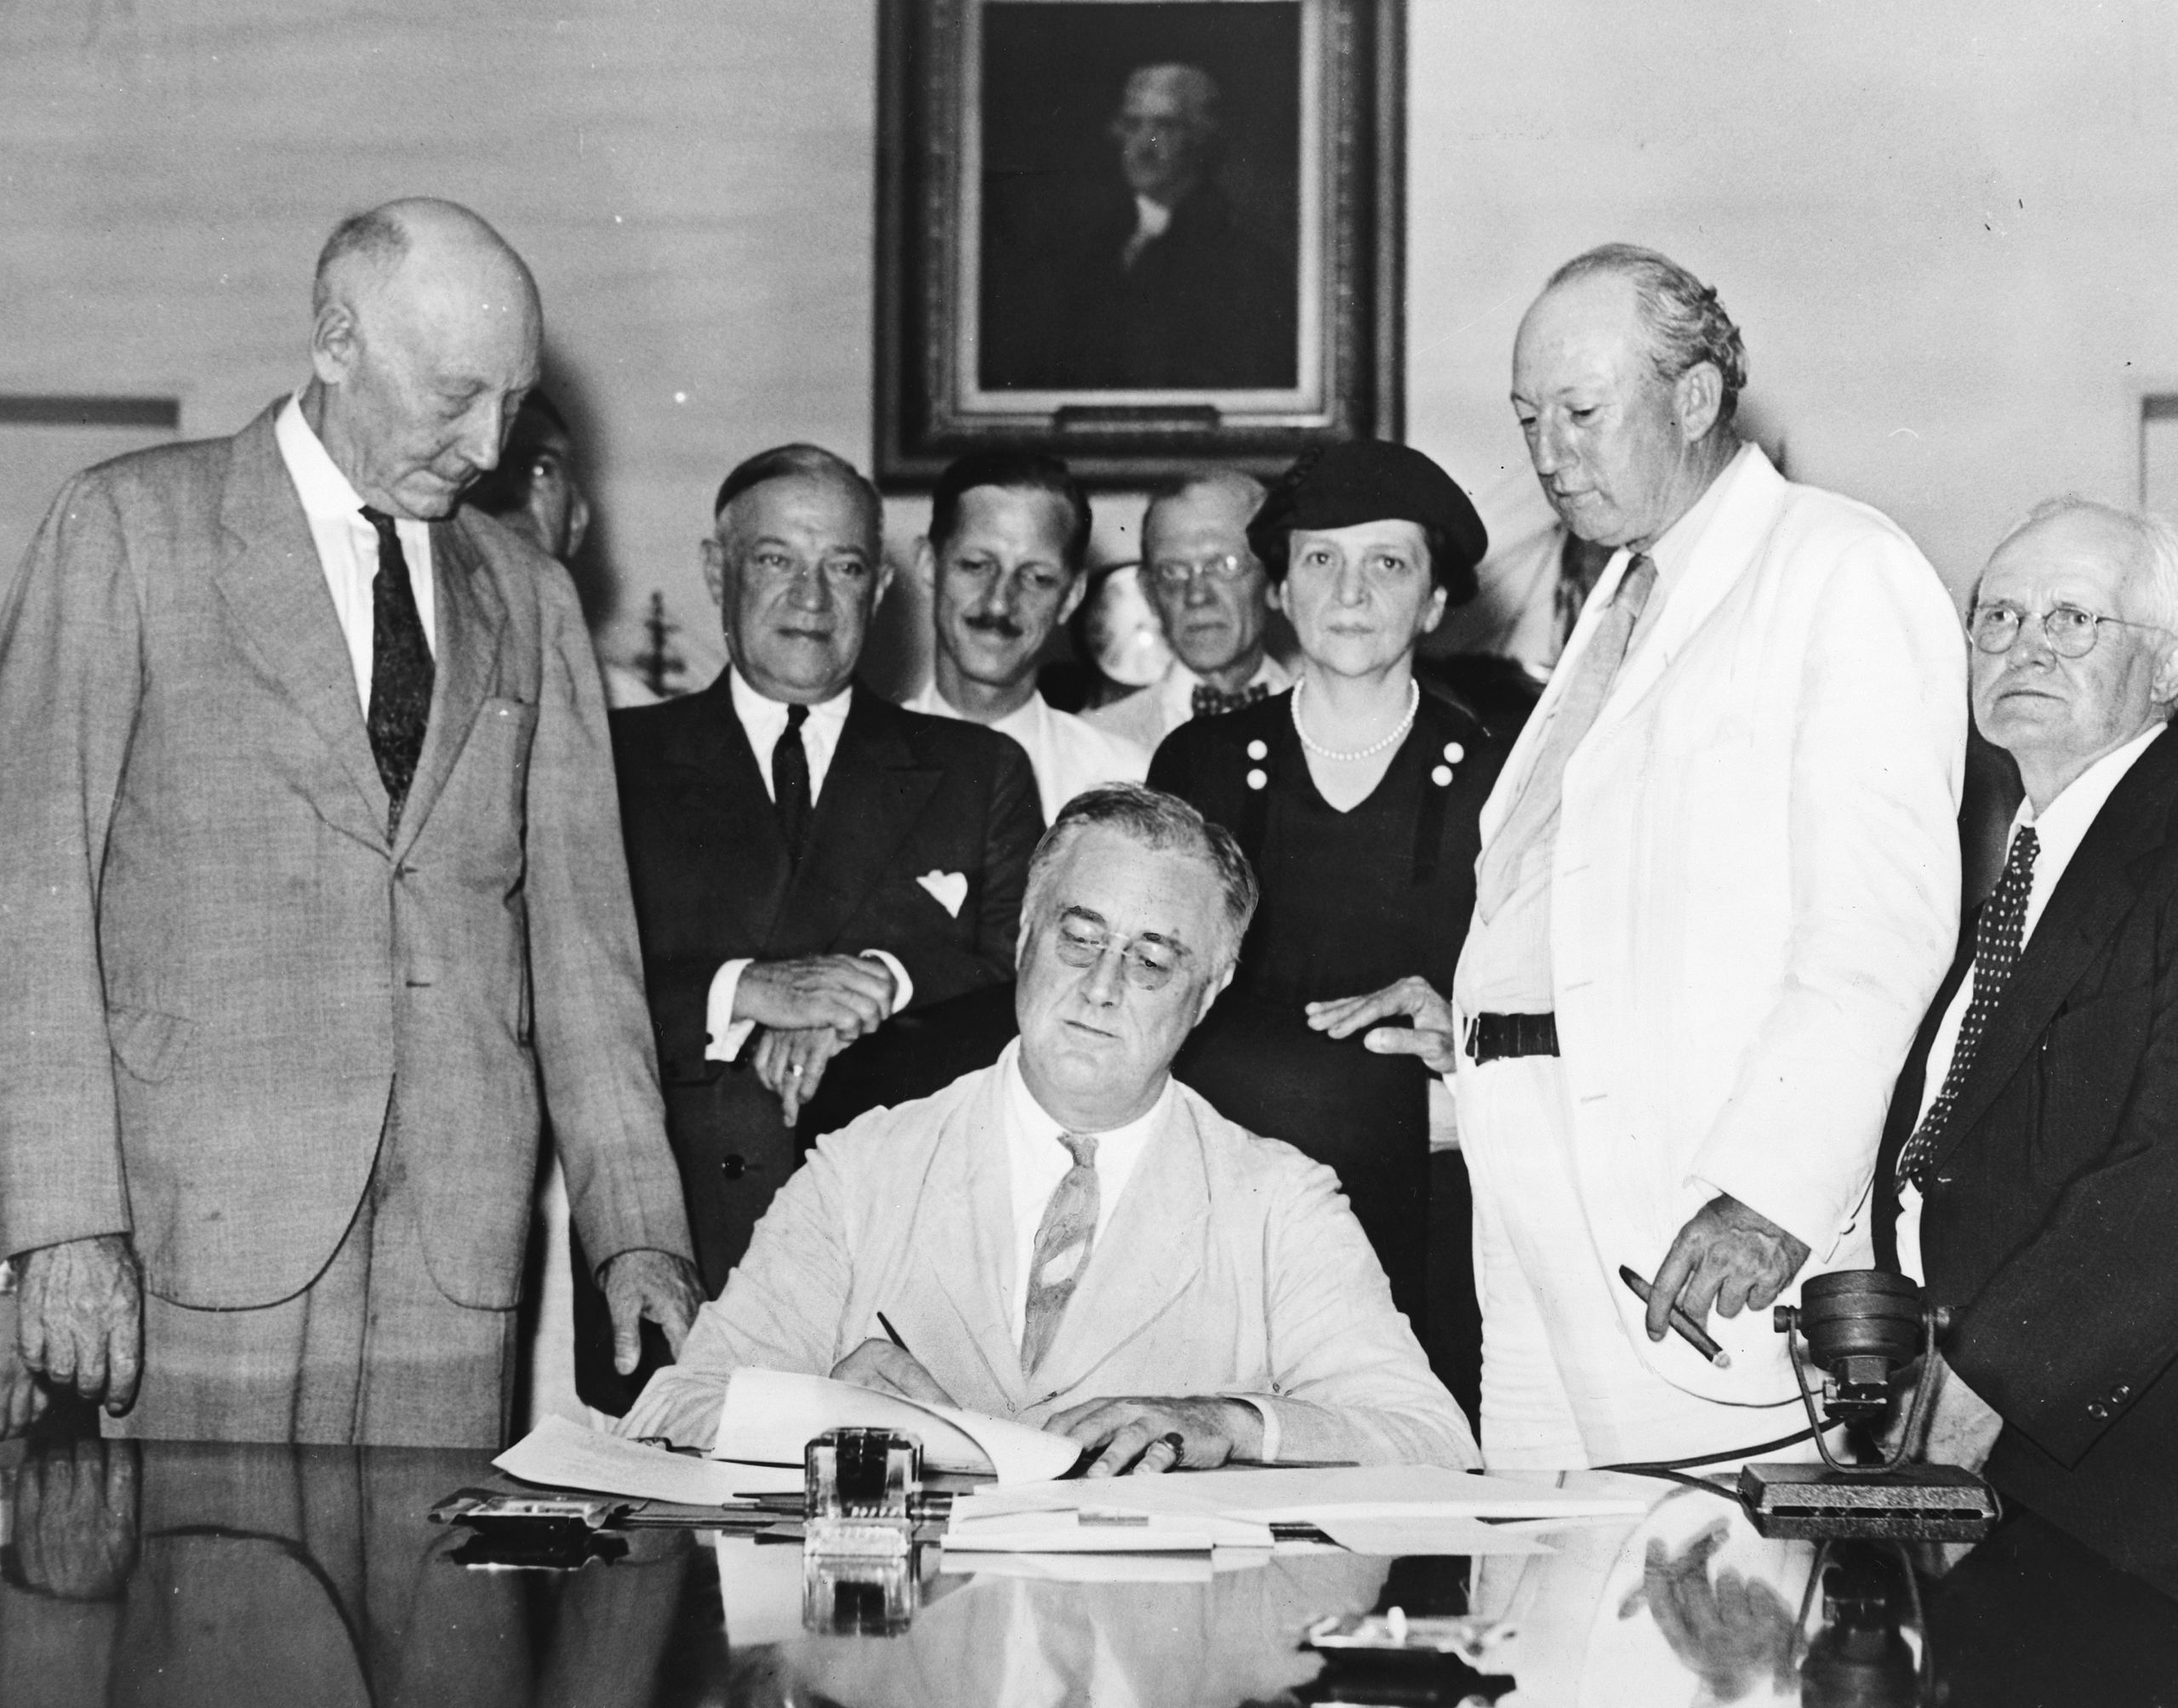
\includegraphics[width = .7\textwidth]{figures/fdr_ssa}\\
Source: \href{https://commons.wikimedia.org/wiki/File:Signing_Of_The_Social_Security_Act.jpg}{Wikimedia}
\end{frame}

\begin{frame}
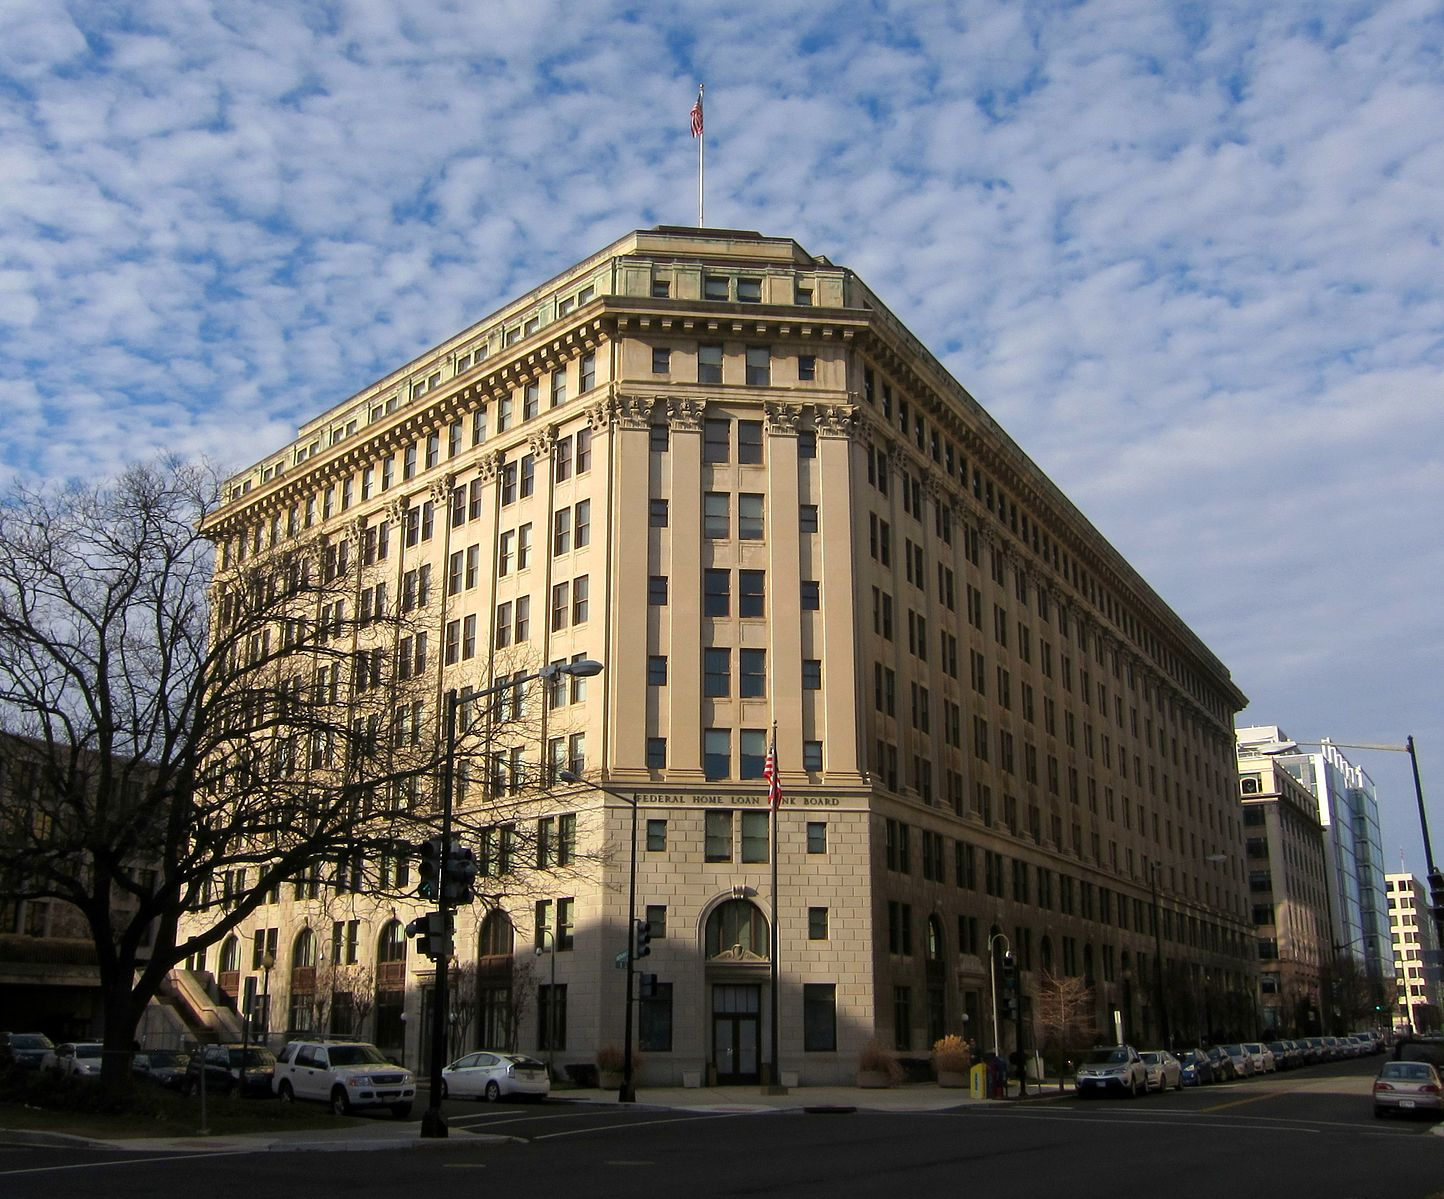
\includegraphics[width = .7\textwidth]{figures/holc_building}\hfill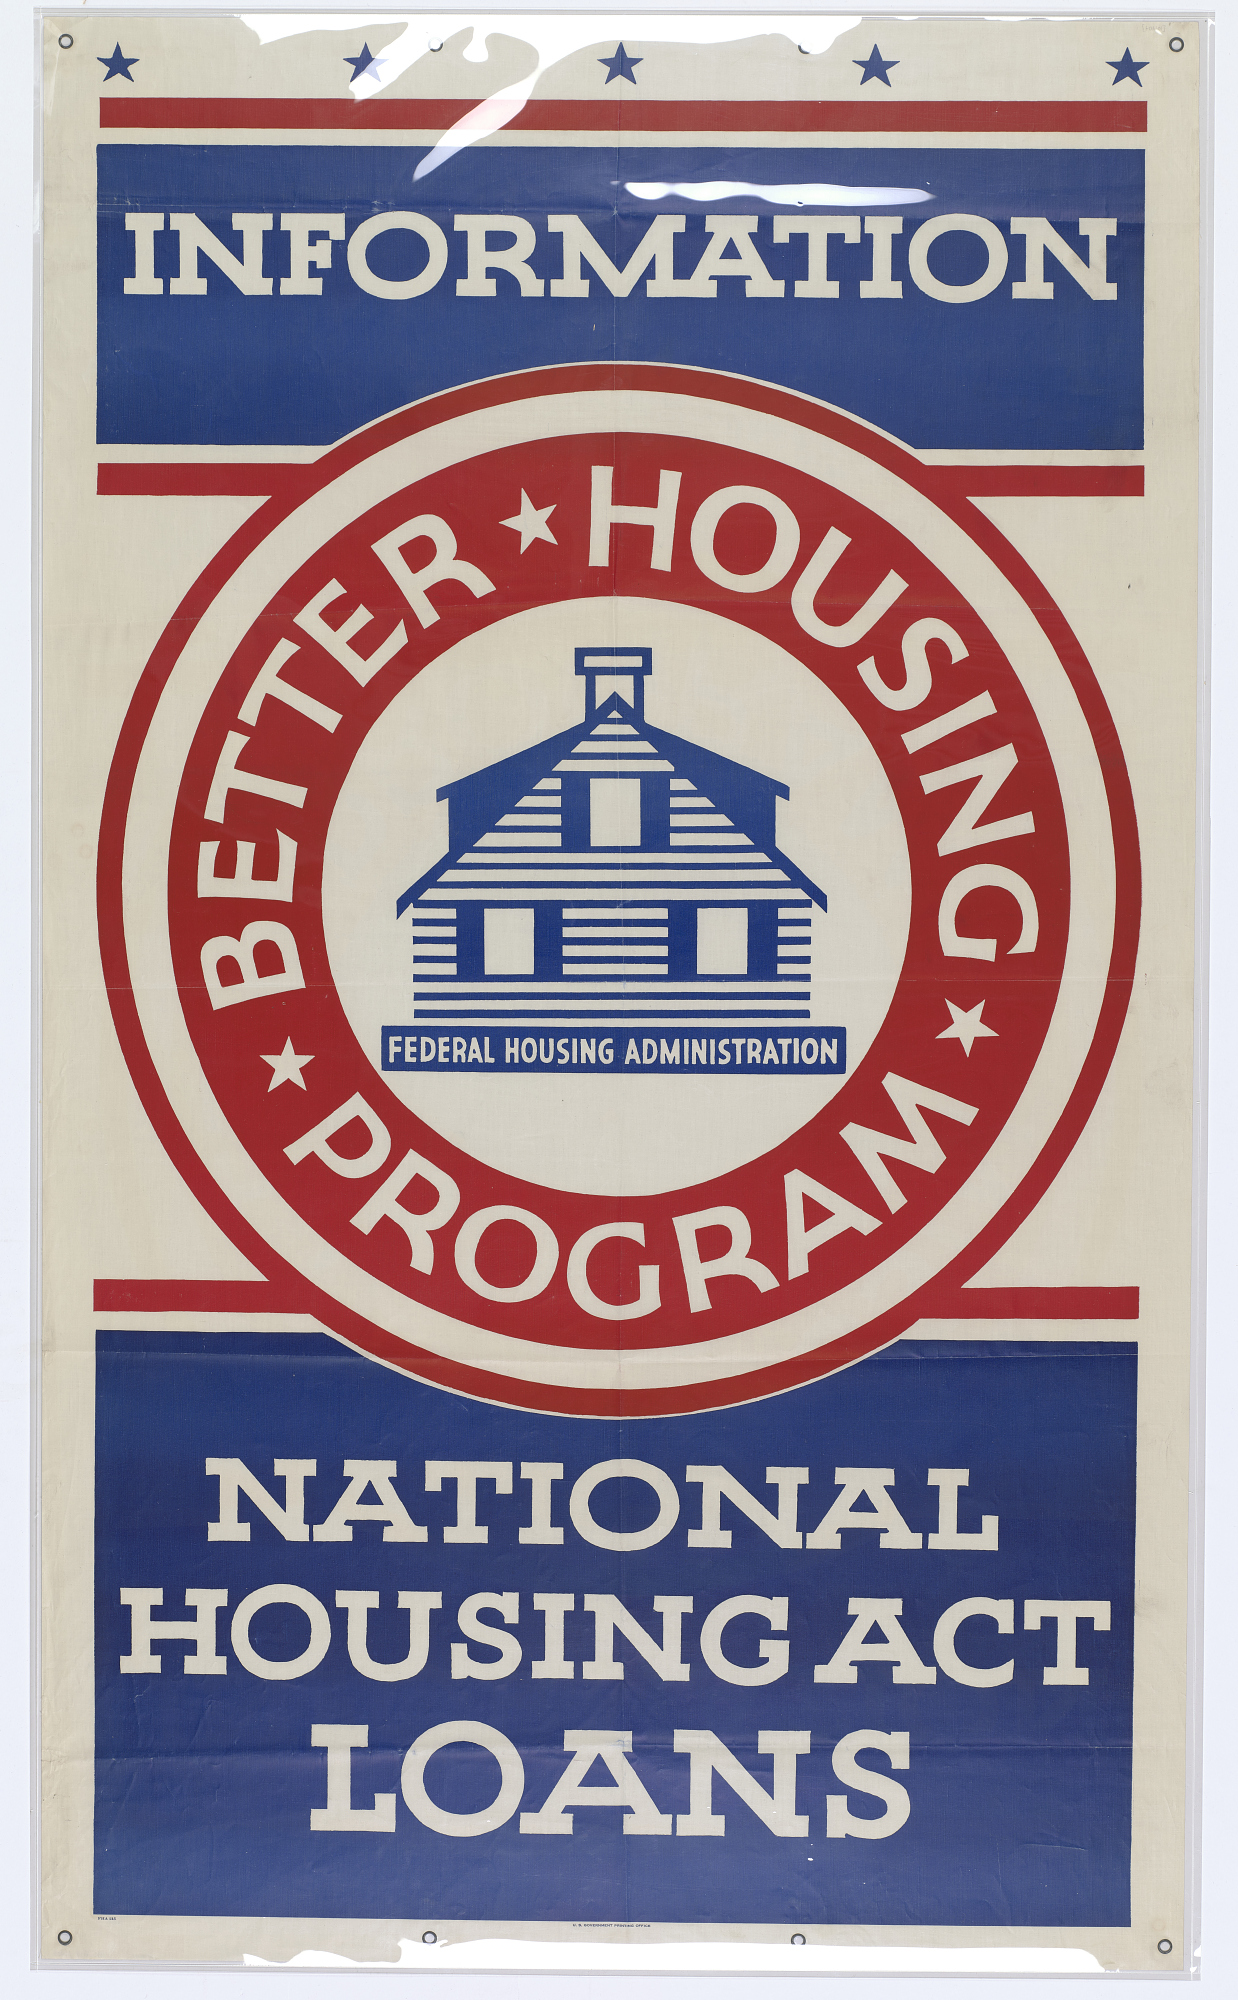
\includegraphics[width = .25\textwidth]{figures/fha_brochure}\\
\begin{footnotesize}
Source: \href{https://commons.wikimedia.org/wiki/File:Federal_Home_Loan_Bank_Board_Building_1.jpg}{Wikimedia} \hfill Source: \href{https://sova.si.edu/details/NMAH.AC.0433\#ref10139}{Smithsonian}
\end{footnotesize}
\end{frame}

\begin{frame}
1933. Half of mortgages in default.\\ \pause
Home Owners Loan Corporation is tasked with saving them\vskip .2in \pause
But who is eligible? \pause \vskip .2in
The agency \textbf{rates neighborhoods}
\begin{itemize}
\item \textcolor{seagreen}{A (most desirable)}
\item \textcolor{blue}{B (less desirable)}
\item \textcolor{mustard}{C (declining)} 
\item \textcolor{red}{D (undesirable)}
\end{itemize} \pause \vskip .2in
%How? \pause\hfill \bred{(redlining)} \pause
Low-income immigrants $\rightarrow$ \textcolor{red}{D grade} \pause \\
Black families $\rightarrow$ \textcolor{red}{D grade}
\vskip .1in \pause
\begin{footnotesize}
Jackson, Kenneth T. \bref{https://books.google.com/books?hl=en&lr=&id=pqRoAgAAQBAJ}{Crabgrass frontier: The suburbanization of the United States.} Oxford University Press, 1987.
\end{footnotesize}
\end{frame}

\begin{frame}
\includegraphics<1>[width = \textwidth]{figures/holc-scan-stlouis} \\
\footnotesize
Maps from Nelson, R. K., Winling, L, et al. (2023).\\\bref{https://dsl.richmond.edu/panorama/redlining}{Mapping Inequality: Redlining in New Deal America.}\\Digital Scholarship Lab.

\end{frame}

\begin{frame}
\begin{tikzpicture}[x = \textwidth]
\node[anchor = west] at (0,.5) {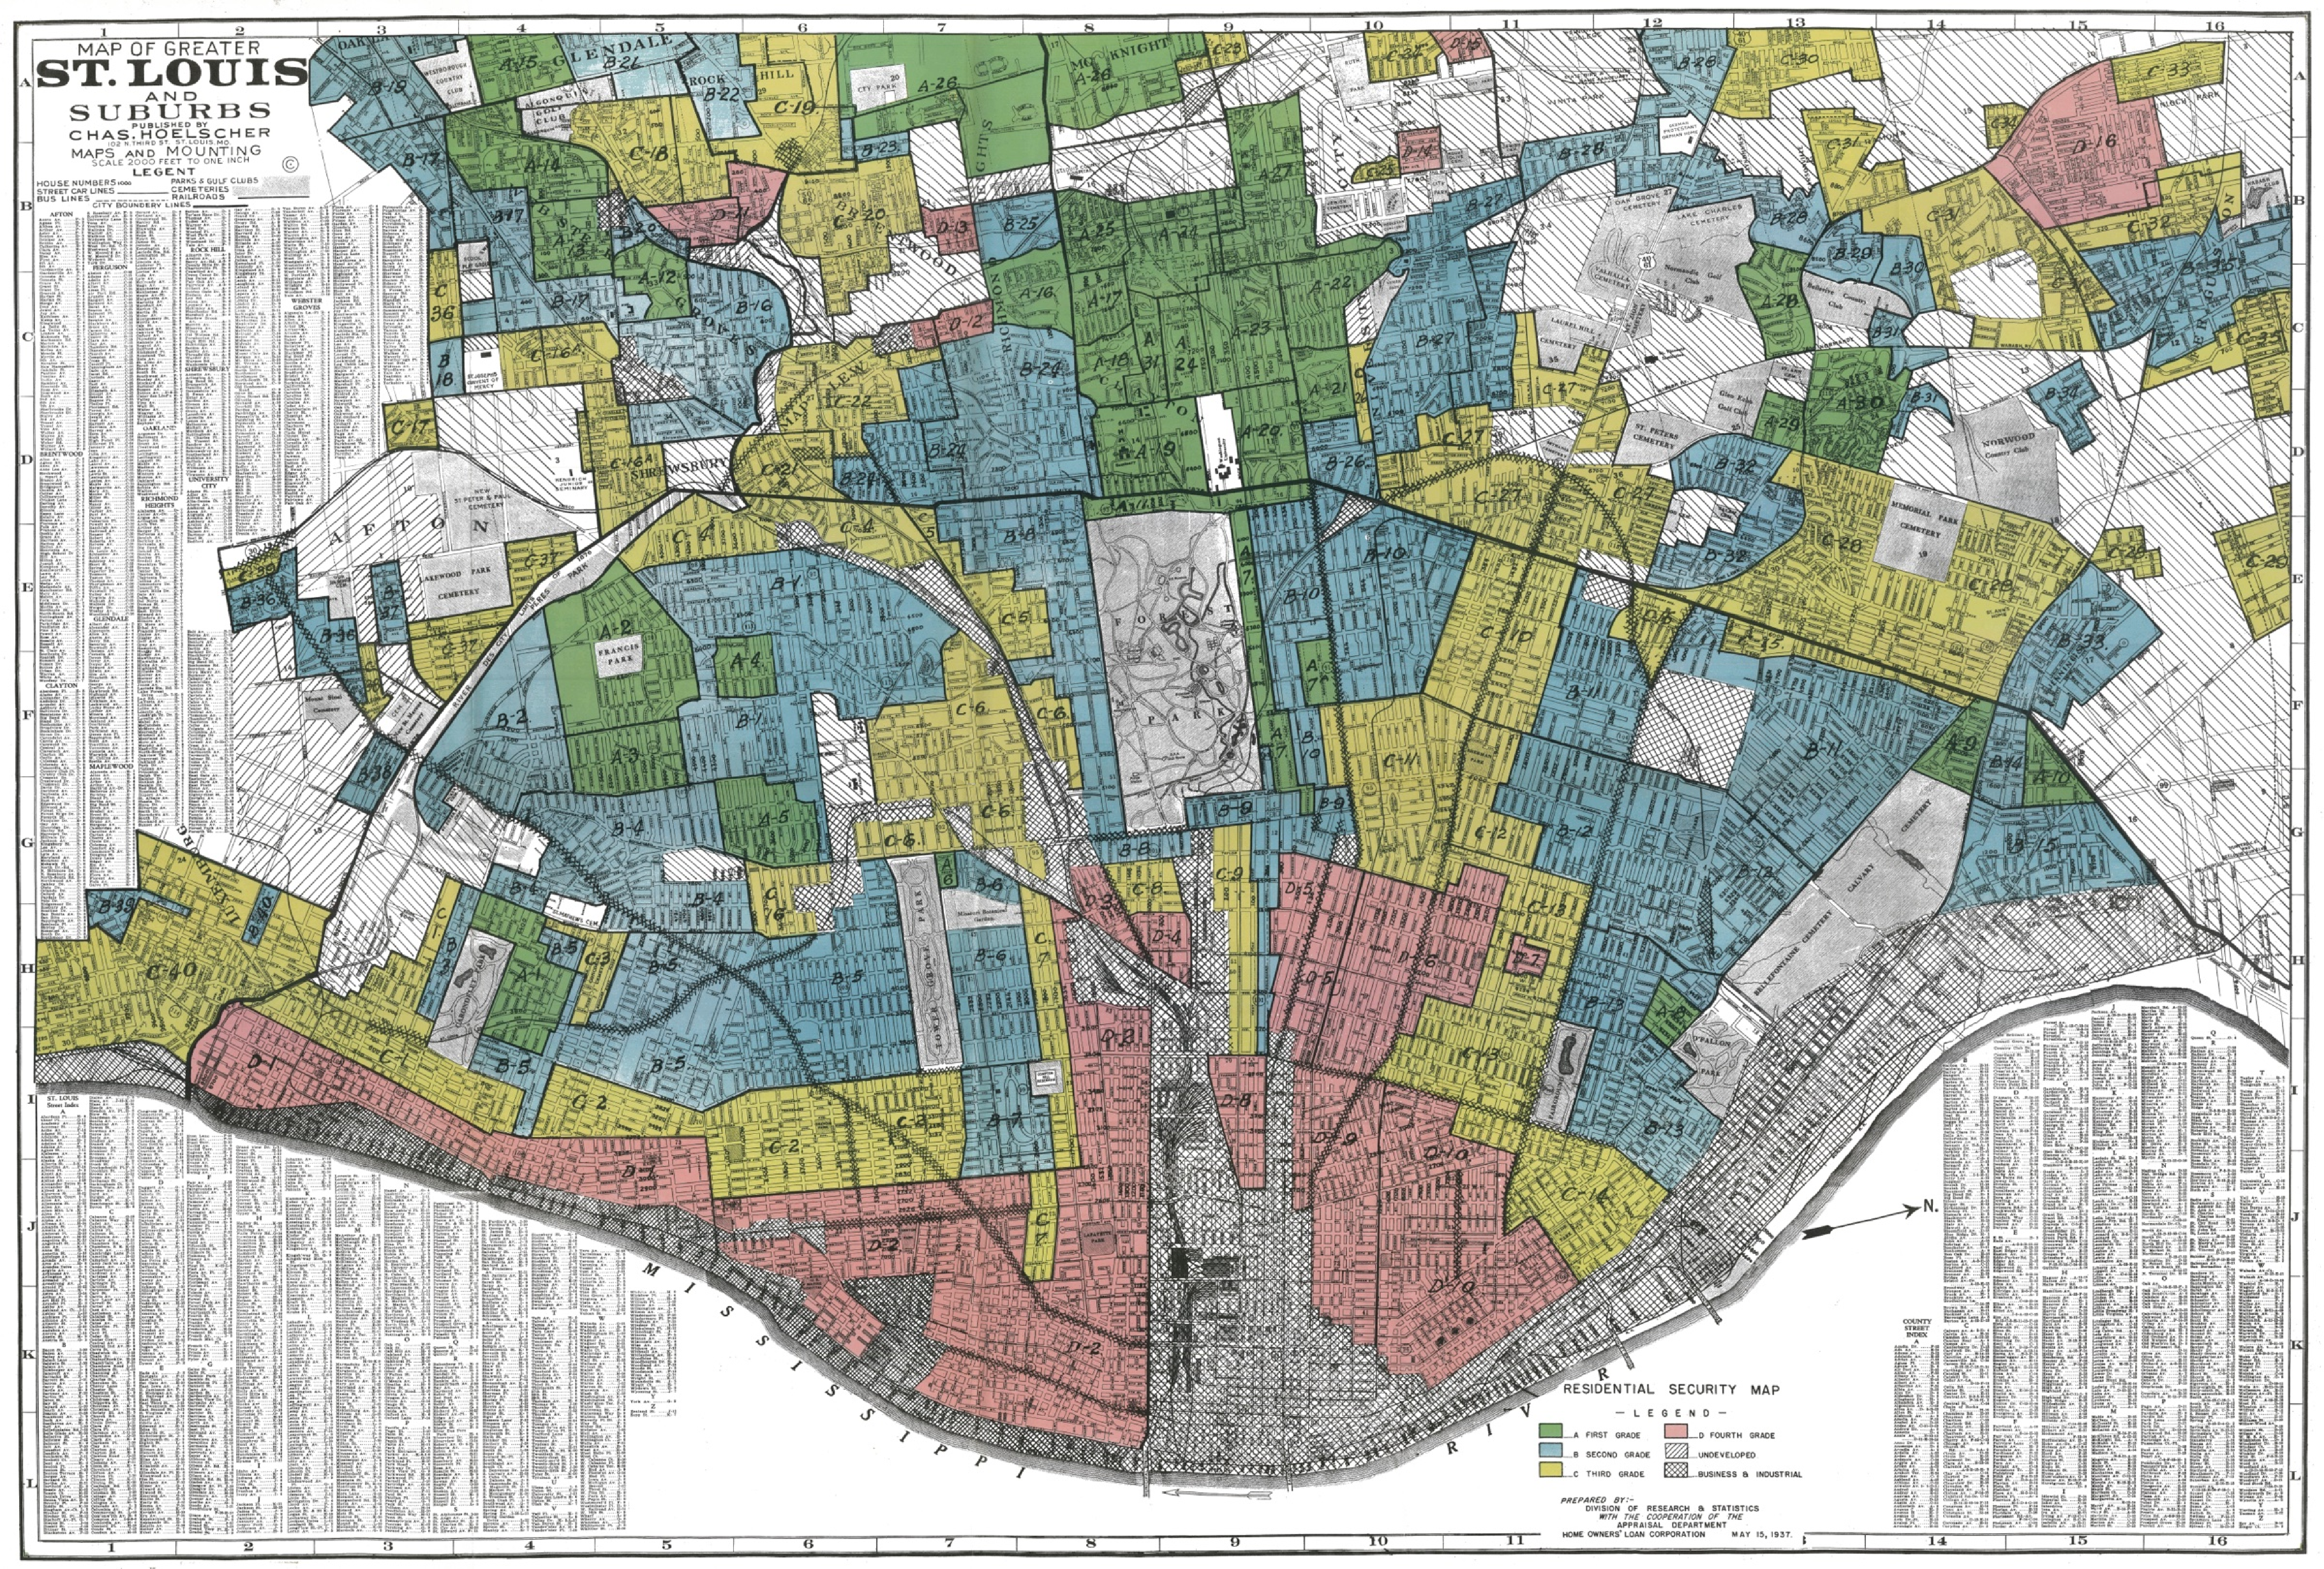
\includegraphics[width = .5\textwidth]{figures/holc-scan-stlouis}};
\node[anchor = north west] (title) at (.6,.9) {\textbf{St. Louis}};
\node[anchor = north west] (text1) at (title.south west) {94,030 African Americans};
\pause
\node[anchor = north west] (text2) at (text1.south west) {0 outside of red areas};
\node[anchor = north west, font = \tiny, gray] at (text2.south west) {Faber 2020, citing Jackson 1985};
\end{tikzpicture}
\end{frame}

\begin{frame}
\includegraphics<1>[height = \textheight]{figures/holc-scan-buffalo}
\end{frame}

\begin{frame}
\includegraphics<1>[height = \textheight]{figures/holc-scan-chicago}
\end{frame}

\begin{frame}
\includegraphics<1>[width = \textwidth]{figures/holc-scan-la}
\end{frame}

\begin{frame}{HOLC loans: 1933--1934}{Source: Faber 2020}
\$3 billion of loans in two years\\
1 out of 10 non-farm, owner-occupied home
\end{frame}

\begin{frame}{1950s and 1960s: Suburbs boomed}{\bref{http://calihist.weebly.com/postwar-era-suburbanization.html}{[image source]}}
\begin{tikzpicture}[x = \textwidth, y = \textheight]
\node[anchor = west] at (0,.5) {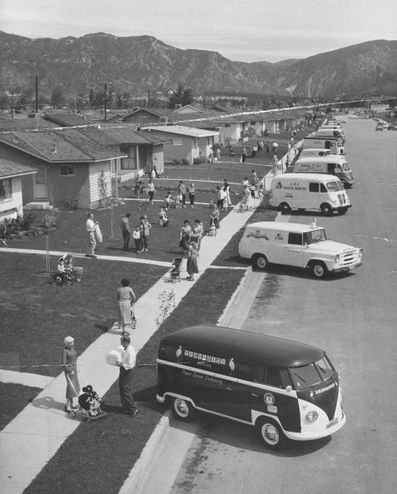
\includegraphics[height = .8\textheight]{figures/suburb}};
\node<2->[anchor = north west] at (.6,.8) {HOLC ended};
\node<3->[anchor = north west, align = left] at (.6,.7) {but the Federal\\Housing Administration\\maintained the\\mapping policy};
\node<4->[anchor = north west, align = left] at (.6,.4) {How did communities\\and homeowners respond?};
\end{tikzpicture}
\end{frame}

\begin{frame}{Local organizations furthered racist policies}
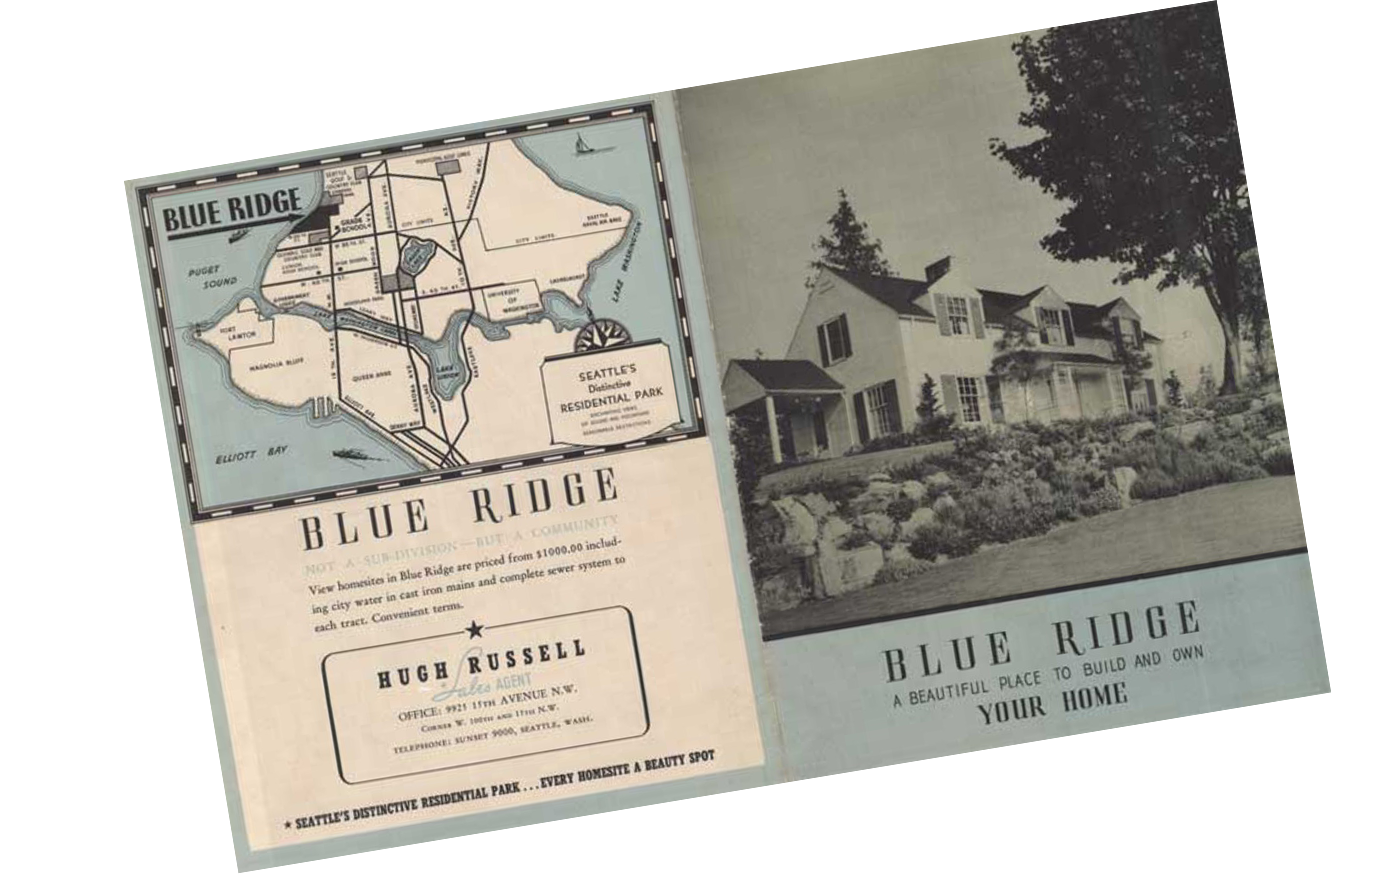
\includegraphics[width = \textwidth]{figures/blueridge_brochure}\\
Source: \href{https://blueridgeseattle.com/about-us/}{Blue Ridge Seattle}
\end{frame}

\begin{frame}{Local organizations furthered racist policies}

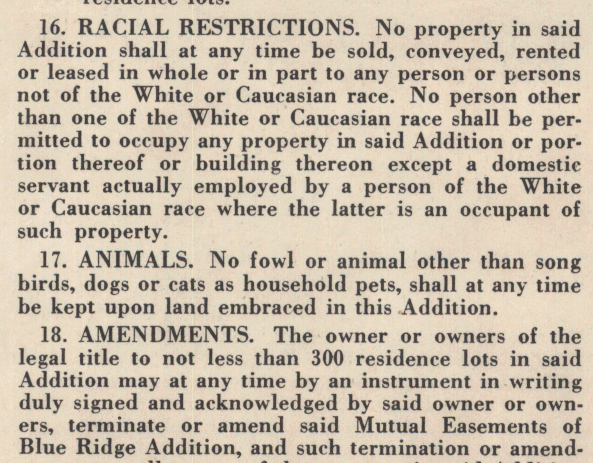
\includegraphics[width = .7\textwidth]{figures/racial_covenant}

\begin{footnotesize}
Source: \href{https://depts.washington.edu/covenants/segregation.shtml}{Civil Rights and Labor History Consortium, University of Washington}
\end{footnotesize}
\end{frame}

\begin{frame}{Fair Housing Act (1968)}{\bref{https://fairhousingnj.org/2019/07/02/the-fair-housing-act/}{image source}, \bref{https://www.history.com/videos/fair-housing-act-of-1968}{video}}

\begin{tikzpicture}[x = \textwidth, y = \textheight]
\node[anchor = south west] at (0,0) {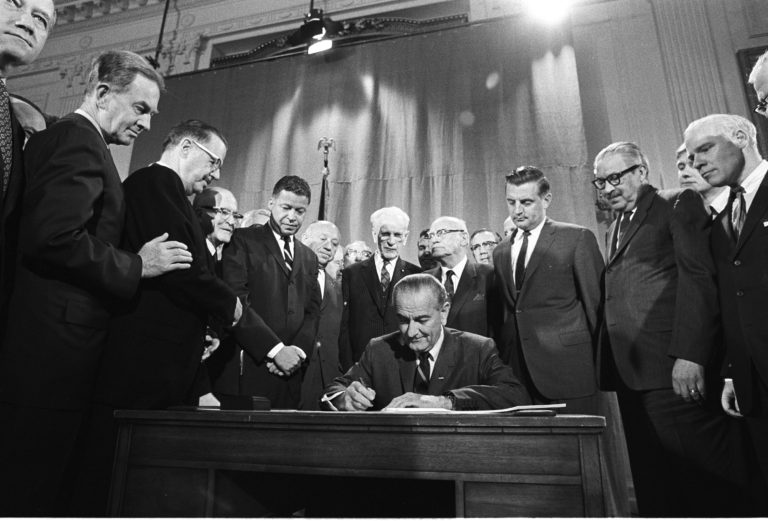
\includegraphics[width = .8\textwidth]{figures/lbj_fha}};
\node[anchor = south east] at (1,0) {
\includegraphics[width = .15\textwidth]{figures/equal_opportunity_logo}};
%\node<2->[anchor = north west, align = left] at (.6,.7) {Prohibited discrimination\\on the basis of\\race, color, religion,\\or national origin\\(more classes added later)};
\end{tikzpicture}

\end{frame}

\begin{frame}{Fair Housing Act (1968)}

\begin{itemize}
\item enforcement was difficult (\bref{https://youtu.be/r3Q6EDNRReg?t=34}{video})
\pause
\item to buy a house, you still needed some wealth \pause
\begin{itemize}
\item white families had gotten that through past home ownership \pause
\item Black families had not \pause
\end{itemize}
\end{itemize}
Segregation and racial inequality\\rooted in the 1930s\\\textbf{persists today}

\end{frame}

\begin{frame}

\huge data science (example 1)

\end{frame}

\begin{frame}

Did HOLC maps cause neighborhoods to become more segregated? \pause \vskip .3in

\includegraphics[width = \textwidth]{figures/faber_title}

\end{frame}

\begin{frame}{Some places were graded by HOLC. Others were not} \pause
\begin{itemize}
\item Policy: Maps required for cities over 40,000 in population \pause
\item Practice
\begin{itemize}
\item 31 cities over 40k that were not mapped
\item 188 cities under 40k that were mapped
\end{itemize}
\end{itemize}
\end{frame}

\begin{frame}{Measuring segregation} \pause

Within each place, there are Census tracts.\vskip .2in \pause
\textbf{Isolation index}\\
On average over African American residents in the place, what is the average proportion of people in their Census tract who are African American? \pause
\begin{itemize}
\item 100\% would be complete segregation
\end{itemize}

\end{frame}

\begin{frame}{The effect of policy on segregation}{Data}

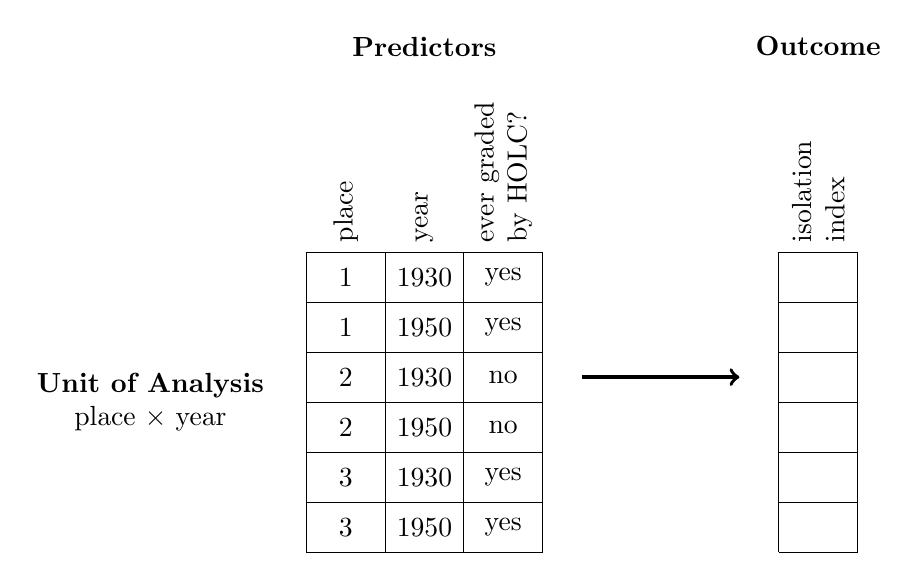
\begin{tikzpicture}[y = .25in]
\node[anchor = east, align = center, outer sep = 12pt] at (-1,3) {\textbf{Unit of Analysis}\\place $\times$ year};
\node[anchor = north, align = center] at (.5,10.5) {\textbf{Predictors}};
\node[anchor = west, rotate = 90] at (-.5,6) {place};
\node[anchor = west, rotate = 90] at (.5,6) {year};
\node[anchor = west, rotate = 90, align = left] at (1.5,6) {ever graded\\by HOLC?};
\draw[ystep = .25in] (-1,0) grid (2,6);
\node at (-.5,5.5) {1};
\node at (-.5,4.5) {1};
\node at (-.5,3.5) {2};
\node at (-.5,2.5) {2};
\node at (-.5,1.5) {3};
\node at (-.5,.5) {3};
\node at (.5,5.5) {1930};
\node at (.5,4.5) {1950};
\node at (.5,3.5) {1930};
\node at (.5,2.5) {1950};
\node at (.5,1.5) {1930};
\node at (.5,.5) {1950};
\node at (1.5,5.5) {yes};
\node at (1.5,4.5) {yes};
\node at (1.5,3.5) {no};
\node at (1.5,2.5) {no};
\node at (1.5,1.5) {yes};
\node at (1.5,.5) {yes};
\node[anchor = north, align = center] at (5.5,10.5) {\textbf{Outcome}};
\node[anchor = west, rotate = 90, align = left] at (5.5,6) {isolation\\index};
\draw[ystep = .25in] (5,0) grid (6,6);
\draw[->, line width = 1.3pt] (2.5,3.5) -- (4.5,3.5);
\end{tikzpicture}

\end{frame}

\begin{frame}{The effect of policy on segregation}{Sample restrictions}

\begin{itemize}
\item place observed in 1920 or 1930, before HOLC
\item Black population over 100
\item at least two Census tracts within the place
\item not missing values on covariates
\end{itemize}

\end{frame}

\begin{frame}

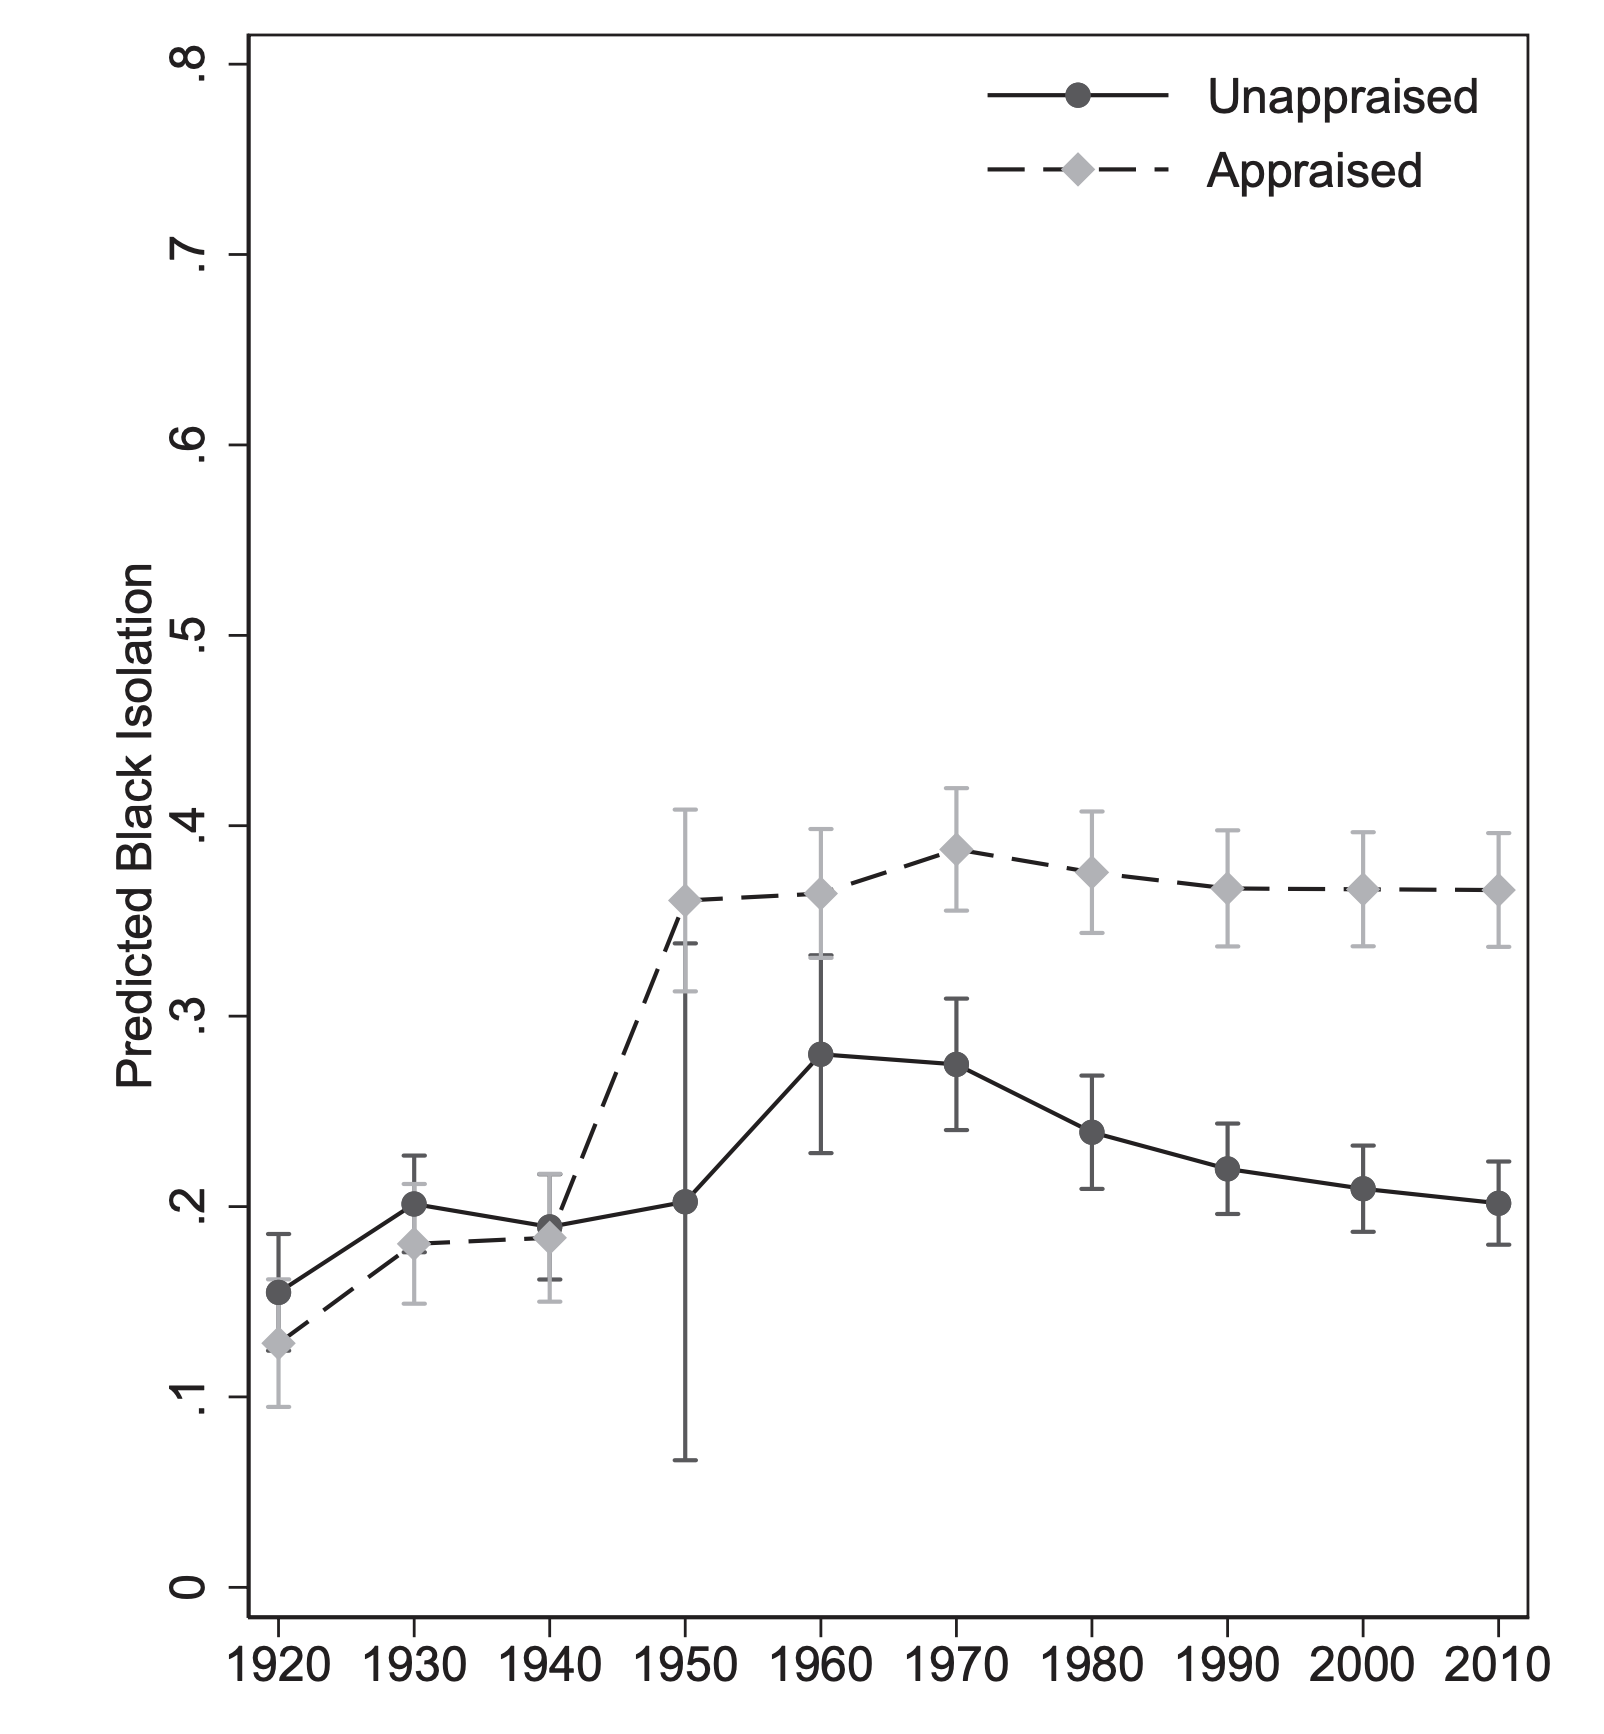
\includegraphics[height = .8\textheight]{figures/faber_fig1}

\begin{footnotesize}
Figure 1 from Faber, J. W. 2020. \bref{https://doi.org/10.1177/0003122420948464}{We built this: Consequences of New Deal era intervention in America’s racial geography.} American Sociological Review, 85(5), 739-775.
\end{footnotesize}
\end{frame}

\begin{frame}

\huge data science (example 2)

\end{frame}


\begin{frame}{Racial Wealth Gap} \pause
In redlined neighborhoods, \pause
\begin{itemize}
\item Hard to sell your home \pause
\item Hard to buy a home \pause
\item Home prices do not rise \pause
\end{itemize} \vskip .2in
In the suburbs, \pause
\begin{itemize}
\item Home ownership skyrockets
\begin{itemize}
\item 44\% owned their home in 1940 \hfill National estimates
\item 62\% in 1960 \hfill from \href{https://www.census.gov/data/tables/time-series/dec/coh-owner.html}{U.S. Census}
\end{itemize} \pause
\item Home prices rise \pause
\item Wealth grows
\end{itemize} \vskip .2in \pause
Oliver, M., \& Shapiro, T. (2013). \bref{https://www.taylorfrancis.com/books/mono/10.4324/9780203707425/black-wealth-white-wealth-melvin-oliver-thomas-shapiro}{Black wealth/white wealth: A new perspective on racial inequality.} Routledge.
\end{frame}

\begin{frame}{Racial Wealth Gap}
{2022 \bref{https://www.federalreserve.gov/econres/aboutscf.htm}{Survey of Consumer Finances}}

\bref{https://sda.berkeley.edu/sdaweb/analysis/?dataset=scfcomb2022}{https://sda.berkeley.edu/sdaweb/analysis/?dataset=scfcomb2022}

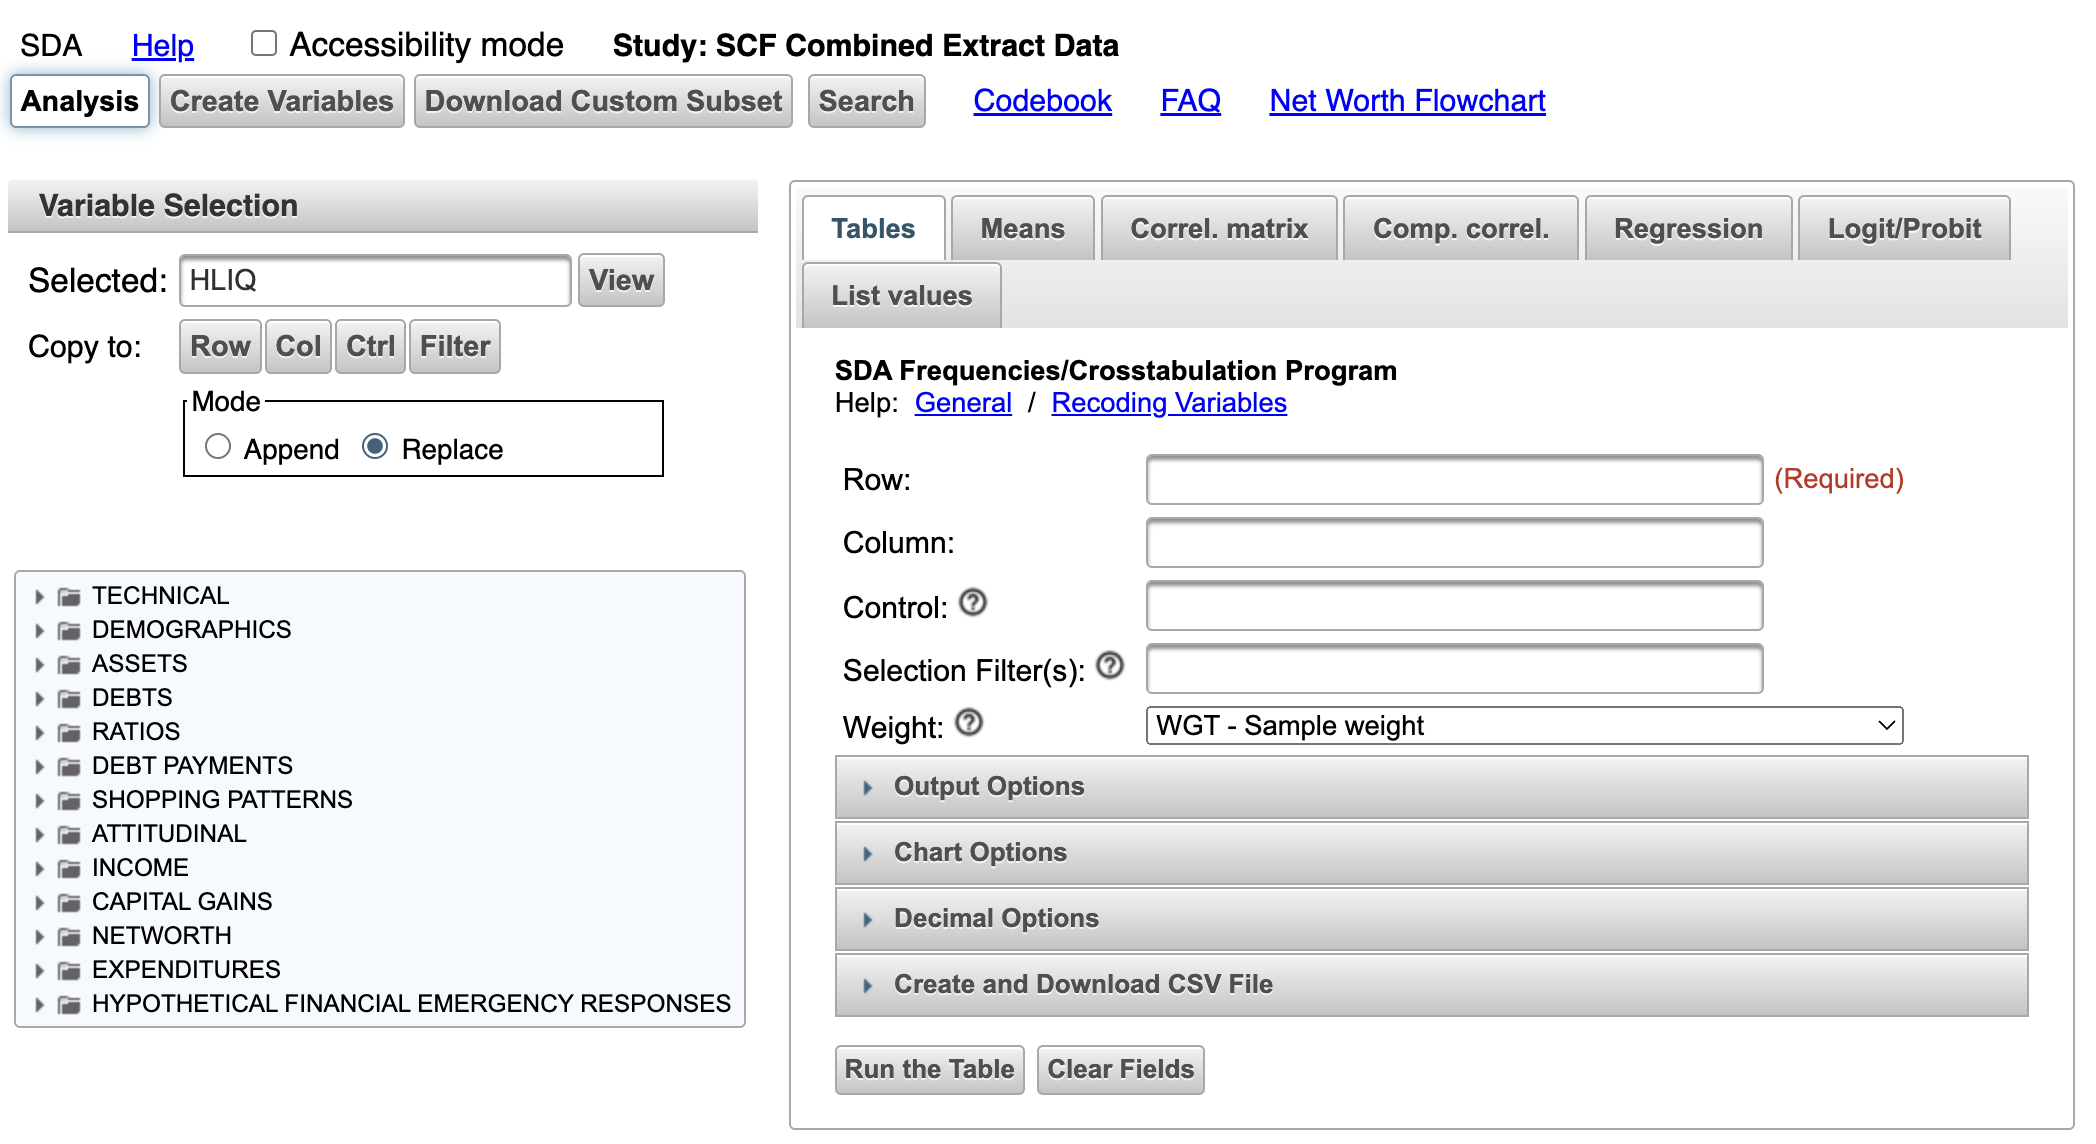
\includegraphics[width = \textwidth]{figures/scf_sda}

\end{frame}


\begin{frame}{Racial Wealth Gap}

2022 Survey of Consumer Finances \bref{https://www.federalreserve.gov/econres/aboutscf.htm}{(link)}
\begin{itemize}
\item unit of analysis: household
\item predictor: race
\item outcome: net worth = assets - debts
\item summarized by the median
\end{itemize} \vskip .2in \pause

White households: \$272,000\\ \pause
Black households: \$49,590\vskip .2in \pause
\begin{center}
\huge Ratio: 5.48
\end{center}
The typical White household has \$5.48 for each \$1 held by the typical Black household

\end{frame}

\begin{frame}{Additional resources}
\footnotesize
\begin{itemize}
\item Oliver, M., \& Shapiro, T. 2013. \bref{https://www.taylorfrancis.com/books/mono/10.4324/9780203707425/black-wealth-white-wealth-melvin-oliver-thomas-shapiro}{Black wealth / white wealth: A new perspective on racial inequality.} Routledge.
\item Faber, J. W. 2020. \bref{https://doi.org/10.1177/0003122420948464}{We built this: Consequences of New Deal era intervention in America’s racial geography.} American Sociological Review, 85(5), 739-775.
\item Massey, D. S., \& Denton, N. A. 1993. \bref{https://www.hup.harvard.edu/catalog.php?isbn=9780674018211}{American apartheid: Segregation and the making of the underclass.} Harvard University Press.
\item Killewald, A., Pfeffer, F. T., \& Schachner, J. N. 2017. \bref{https://doi.org/10.1146/annurev-soc-060116-053331}{Wealth inequality and accumulation.} Annual Review of Sociology, 43, 379.
\end{itemize}
\end{frame}

\goalsframe

\end{document}

